\section{Arquitectura de la aplicación}
La arquitectura utilizada en esta aplicación se basa en un sistema cliente servidor donde el cliente, mediante conexión a internet, realiza peticiones al servidor y se queda a la espera de la respuesta  para realizar las diferentes acciones solicitadas. En la figura \ref{fig:arquitectura_del_sistema} se puede ver una representación gráfica de este sistema. 

\begin{figure}[H]
    \centering
    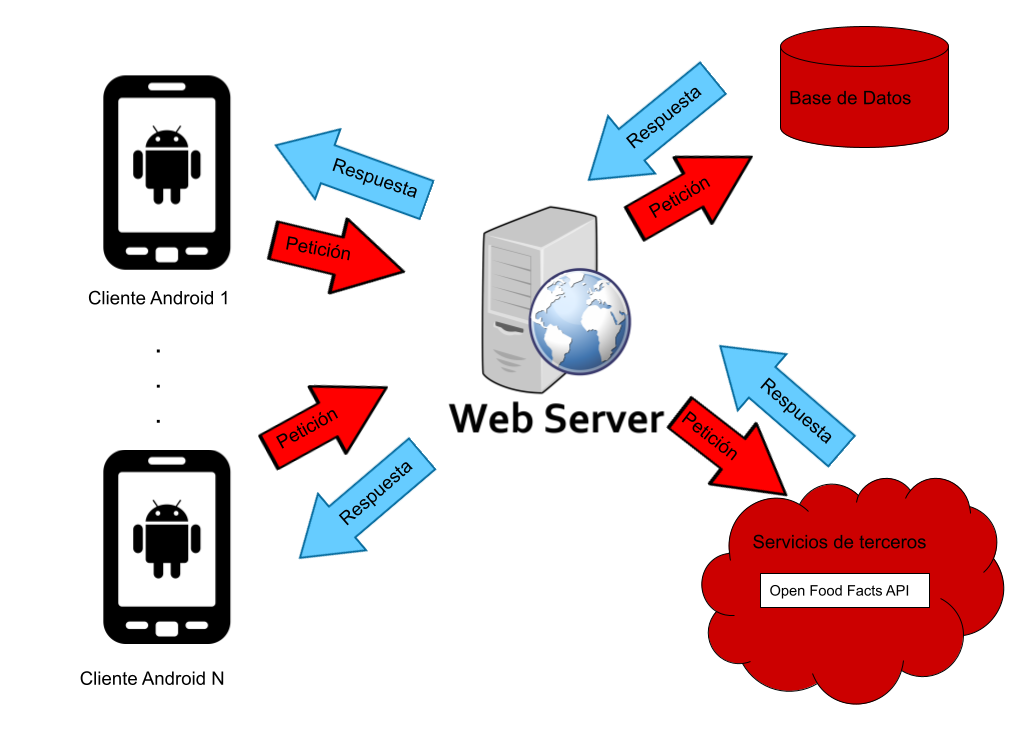
\includegraphics[width=0.9\textwidth]{Images/Capitulo6/arquitectura.png}
    \caption{Esquema de la arquitectura de la aplicación}
    \label{fig:arquitectura_del_sistema}
\end{figure}

Como se puede observar en la figura \ref{fig:arquitectura_del_sistema}, el usuario necesita tener su dispositivo conectado a internet en todo momento para poder realizar peticiones al servidor web. El servidor a su vez se conecta con los diferentes proveedores de servicios, ya sea a la base de datos de la aplicación o a la API encargada de de obtener los alimentos.
% Con el fin de tener todos los datos actualizados, cuando un usuario realiza una petición al servidor, este se queda permanentemente escuchando hasta que dicho cliente decida realizar otra acción diferente. 
En este proyecto el servidor web enviará y recibirá las peticiones de manera asíncrona para mejorar la eficiencia a la hora de comunicarse con los diferentes elementos del sistema.
